%Version 3 October 2023
% See section 11 of the User Manual for version history
%
%%%%%%%%%%%%%%%%%%%%%%%%%%%%%%%%%%%%%%%%%%%%%%%%%%%%%%%%%%%%%%%%%%%%%%
%%                                                                 %%
%% Please do not use \input{...} to include other tex files.       %%
%% Submit your LaTeX manuscript as one .tex document.              %%
%%                                                                 %%
%% All additional figures and files should be attached             %%
%% separately and not embedded in the \TeX\ document itself.       %%
%%                                                                 %%
%%%%%%%%%%%%%%%%%%%%%%%%%%%%%%%%%%%%%%%%%%%%%%%%%%%%%%%%%%%%%%%%%%%%%

%%\documentclass[referee,sn-basic]{sn-jnl}% referee option is meant for double line spacing

%%=======================================================%%
%% to print line numbers in the margin use lineno option %%
%%=======================================================%%

%%\documentclass[lineno,sn-basic]{sn-jnl}% Basic Springer Nature Reference Style/Chemistry Reference Style

%%======================================================%%
%% to compile with pdflatex/xelatex use pdflatex option %%
%%======================================================%%

%%\documentclass[pdflatex,sn-basic]{sn-jnl}% Basic Springer Nature Reference Style/Chemistry Reference Style


%%Note: the following reference styles support Namedate and Numbered referencing. By default the style follows the most common style. To switch between the options you can add or remove `Numbered` in the optional parenthesis. 
%%The option is available for: sn-basic.bst, sn-vancouver.bst, sn-chicago.bst%  
 
%%\documentclass[sn-nature]{sn-jnl}% Style for submissions to Nature Portfolio journals
%%\documentclass[sn-basic]{sn-jnl}% Basic Springer Nature Reference Style/Chemistry Reference Style
\documentclass[sn-mathphys-num]{sn-jnl}% Math and Physical Sciences Numbered Reference Style 
%%\documentclass[sn-mathphys-ay]{sn-jnl}% Math and Physical Sciences Author Year Reference Style
%%\documentclass[sn-aps]{sn-jnl}% American Physical Society (APS) Reference Style
%%\documentclass[sn-vancouver,Numbered]{sn-jnl}% Vancouver Reference Style
%%\documentclass[sn-apa]{sn-jnl}% APA Reference Style 
%%\documentclass[sn-chicago]{sn-jnl}% Chicago-based Humanities Reference Style

\graphicspath{{figs}}

%%%% Standard Packages
%%<additional latex packages if required can be included here>

\usepackage{graphicx}%
\usepackage{multirow}%
\usepackage{amsmath,amssymb,amsfonts}%
\usepackage{amsthm}%
\usepackage{mathrsfs}%
\usepackage[title]{appendix}%
\usepackage{xcolor}%
\usepackage{textcomp}%
\usepackage{manyfoot}%
\usepackage{booktabs}%
\usepackage{algorithm}%
\usepackage{algorithmicx}%
\usepackage{algpseudocode}%
\usepackage{listings}%
%%%%

\newcommand{\myfigref}[2]{~\ref{#1}.\subref{#2}}% <---- a new macro for referring to a subfigure
\usepackage{subfig} % for subfigures
\usepackage{wrapfig}

%%%%%=============================================================================%%%%
%%%%  Remarks: This template is provided to aid authors with the preparation
%%%%  of original research articles intended for submission to journals published 
%%%%  by Springer Nature. The guidance has been prepared in partnership with 
%%%%  production teams to conform to Springer Nature technical requirements. 
%%%%  Editorial and presentation requirements differ among journal portfolios and 
%%%%  research disciplines. You may find sections in this template are irrelevant 
%%%%  to your work and are empowered to omit any such section if allowed by the 
%%%%  journal you intend to submit to. The submission guidelines and policies 
%%%%  of the journal take precedence. A detailed User Manual is available in the 
%%%%  template package for technical guidance.
%%%%%=============================================================================%%%%

%% as per the requirement new theorem styles can be included as shown below
\theoremstyle{thmstyleone}%
\newtheorem{theorem}{Theorem}%  meant for continuous numbers
%%\newtheorem{theorem}{Theorem}[section]% meant for sectionwise numbers
%% optional argument [theorem] produces theorem numbering sequence instead of independent numbers for Proposition
\newtheorem{proposition}[theorem]{Proposition}% 
%%\newtheorem{proposition}{Proposition}% to get separate numbers for theorem and proposition etc.

\theoremstyle{thmstyletwo}%
\newtheorem{example}{Example}%
\newtheorem{remark}{Remark}%

\theoremstyle{thmstylethree}%
\newtheorem{definition}{Definition}%

\raggedbottom
%%\unnumbered% uncomment this for unnumbered level heads

% transpose
\newcommand{\T}{^{\mathsf{T}}}

\begin{document}

\title{Forecasting fMRI Images From Video Sequences: Linear Model Analysis}

%%=============================================================%%
%% GivenName	-> \fnm{Joergen W.}
%% Particle	-> \spfx{van der} -> surname prefix
%% FamilyName	-> \sur{Ploeg}
%% Suffix	-> \sfx{IV}
%% \author*[1,2]{\fnm{Joergen W.} \spfx{van der} \sur{Ploeg} 
%%  \sfx{IV}}\email{iauthor@gmail.com}
%%=============================================================%%

\author*[1]{\fnm{Daniil} \sur{Dorin}}\email{dddaniil007@gmail.com}
\equalcont{These authors contributed equally to this work.}

\author[2]{\fnm{Nikita} \sur{Kiselev}}\email{n.kiselev@innopolis.ru}
\equalcont{These authors contributed equally to this work.}

\author[3]{\fnm{Andrey} \sur{Grabovoy}}\email{grabovoy@ap-team.ru}

\author[1]{\fnm{Vadim} \sur{Strijov}}\email{strijov@gmail.com}

\affil[1]{\orgname{Forecsys}, \city{Moscow}, \country{Russia}}

\affil[2]{\orgname{Research Center for Artificial Intelligence, Innopolis University}, \city{Innopolis}, \country{Russia}}
\affil[3]{\orgname{Antiplagiat Company}, \city{Moscow}, \country{Russia}}

%%==================================%%
%% Sample for unstructured abstract %%
%%==================================%%

% \abstract{The issue of reconstructing the relationship between functional magnetic resonance imaging (fMRI) sensor readings and human perception of the external is investigated. The study analyzes the dependence between the fMRI images and the videos viewed by individuals. Based on this analysis, a method is proposed for approximating the fMRI readings using the video sequence. The method is based on the assumption that there is a time-invariant hemodynamic response to changes in blood oxygen levels. A linear model is constructed for each individual voxel in the fMRI image, assuming that the image sequence follows a Markov property. To test the proposed method, a computational experiment was conducted on a dataset collected during tomographic examinations of a large number of individuals. The performance of the method was evaluated based on the experimental data, and hypotheses were tested regarding the invariance of the model weights and the correctness of the method.}

\abstract{
Over the past few decades, a variety of significant scientific breakthroughs have been achieved in the fields of brain encoding and decoding using the functional magnetic resonance imaging (fMRI). Many studies have been conducted on the topic of human brain reaction to visual stimuli. However, the relationship between fMRI images and video sequences viewed by humans remains complex and is often studied using large transformer models. In this paper, we investigate the correlation between videos presented to participants during an experiment and the resulting fMRI images. To achieve this, we propose a method for creating a linear model that predicts changes in fMRI signals based on video sequence images. A linear model is constructed for each individual voxel in the fMRI image, assuming that the image sequence follows a Markov property. Through the comprehensive qualitative experiments, we demonstrate the relationship between the two time series. We hope that our findings contribute to a deeper understanding of the human brain's reaction to external stimuli and provide a basis for future research in this area.
}

\keywords{neuroimaging, fMRI, video sequences, correlation analysis, hypothesis testing, linear model, forecasting}

%%\pacs[JEL Classification]{D8, H51}

%%\pacs[MSC Classification]{35A01, 65L10, 65L12, 65L20, 65L70}

\maketitle

\section{Introduction}

The study of the human brain has long been a subject of interest for scientists~\cite{zhu2024jointly, sudha2024dynamically,samokhina2022classification, tigga2022efficacy}. One specialized technique for brain research is functional magnetic resonance imaging (fMRI)~\cite{Glover2011}, which allows researchers to identify which regions of the brain are activated by external stimuli. A significant number of studies have focused on analyzing visual stimuli presented during fMRI scans~\cite{ozcelik2023naturalscenereconstructionfmri,THIRION20061104,kamitani2005,haynes2005,COX2003261,haxby2001}. These studies aim to either predict or generate images that the subject may have seen, based on the results of the tomographic scan.

Additionally, some studies have used videos as external stimuli~\cite{chen2023cinematicmindscapeshighqualityvideo,Lan2023SeeingTT,Sun2024NeuroCineDV}. However, this approach presents a computational challenge due to the large amount of data involved. As a result, researchers have recommended using large transformer models for video prediction tasks. However, not all practical implications require such a detailed analysis of the dependency under investigation.

In this paper, we investigate the correlation between a video sequence presented to a patient and the images obtained from their fMRI examination. Therefore, we propose a technique for developing a linear model between two multidimensional time series, see Figure~\ref{fig:scheme}. We note that the constructed method is convenient precisely for analyzing the correlation between them, while high-quality fMRI images forecasting is a more difficult task and requires a more complex architecture.

\begin{figure}[h!]
\centering
\includegraphics[width=\textwidth]{scheme.pdf}
\caption{Overview of our proposed forecasting method. Preprocessing stage (left one) involves the image features extraction using the pre-trained image encoder model. fMRI images are preprocessed using normalizing techniques. Forecasting stage (right one) comprises a multi-dimensional linear model, which maps the video frame embedding to the difference between two sequential tensors.}
\label{fig:scheme}
\end{figure}

The fundamental assumption in this instance is that the series of fMRI images possesses the Markov property, meaning that each subsequent image is dependent solely on the preceding one. The model that we present enables us to forecast the subsequent fMRI image given the preceding image, as well as the video presented to the individual at that time. By employing this autoregressive approach, we can reconstruct the entire sequence of magnetic resonance images based on the viewed video. Proposed technique allows us to investigate the dependence of the reactions of individual brain parts on the objects in the video frame. 

We conduct an in-depth empirical analysis of the suggested method for forecasting the time series of fMRI images. For this purpose, we utilize the dataset~\cite{Berezutskaya2022} that includes both a series of tomographic images and annotated video segments. We analyze the relationship between the two time series by testing various hypotheses. Based on existing medical research~\cite{anderson2006}, we have identified the region responsible for visual processing and used it to estimate the error in our proposed forecasting method. This enables us to significantly enhance the analysis of the connection between the two variables.

Our contributions can be summarized as follows:
\begin{itemize}
\item We present a linear autoregressive model for predicting fMRI image sequences based on the video stimuli. This model leverages the Markov property assumption for fMRI images.
\item We demonstrate the validity of our theoretical results through empirical studies on the available dataset, showing that the proposed model can effectively predict future fMRI images given the preceding image and the corresponding video frame. We quantify the prediction accuracy within a specific brain region associated with visual processing, providing insights into the model's performance.
\item We highlight the implications of our findings for understanding the dynamic relationship between visual stimuli and brain activity. This approach offers a simplified yet effective method for analyzing fMRI data in the context of video stimuli, potentially opening avenues for future research in areas such as cognitive neuroscience and brain-computer interfaces.
\end{itemize}

\section{Related Work}

A set of techniques used to visualize the structure and function of the human brain is called \textit{neurovisualization}. Neuroimaging \cite{puras2014neurovisualization} techniques, such as electrocardiography (ECG), computed tomography (CT), magnetic resonance imaging (MRI), and functional magnetic resonance imaging (fMRI), are used to study the brain and detect diseases and mental disorders \cite{zhu2024jointly, sudha2024dynamically, tigga2022efficacy}.

\textit{Functional magnetic resonance imaging}, or \textit{fMRI}, is a type of magnetic resonance imaging  that measures changes in blood flow in the brain. These changes are caused by neural activity \cite{Glover2011} and occur with a delay of 4--8 seconds \cite{Bandettini1992}, due to the time it takes for the vascular system to respond to the brain's demand for glucose \cite{Ogawa1990, LEBIHAN1995231, Logothetis2003}. This delayed response is essential for accurate fMRI measurements, as it allows for the detection of neural activity that occurs over a longer period of time.

In fMRI imaging, sequences of echo-planar imaging (EPI) are used \cite{Connelly1993, Kwong1992, Ogawa1992}. The processing of areas with varying signal intensities, depending on the method of activation and the type of artifact, is carried out using specialized methods and software \cite{Bandettini1992, BAUDENDISTEL1995701, COX1996162}. The processed results are then formalized as activation maps, which can be combined with the localization of anatomical structures in the cerebral cortex.

The fMRI technique plays a significant role in neuroimaging, although it has some significant limitations. The works of \cite{menon1999spatial} and \cite{logothetis2008we} discuss the temporal and spatial resolution of fMRI, with the latter emphasizing the significant disadvantage of temporal resolution. Another limitation of fMRI is the inevitable noise associated with movement, such as that caused by the heartbeat and respiration of the subject, as well as thermal fluctuations of the scanner itself. In the paper \cite{1804.10167}, graph-based techniques are proposed to address these issues and demonstrate their effectiveness in tasks such as epilepsy and depression detection. These methods aim to suppress the noise mentioned above and improve the accuracy of the results.

In fMRI, the participant is given a variety of tasks and external stimuli, which induce activation of specific areas of the brain. These stimuli include movements of fingers and limbs \cite{Roux1998, Papke1999}, image finding and examination of a chessboard \cite{Engel1994, Schneider1994}, listening to non-specific noises, and reading single words or coherent text \cite{Binder1994, Dymarkowski1998}. Changes in brain activity during the fMRI examination could also be caused by watching a video  \cite{decety1997brain}, which is the focus of this study.

The most well-known video processing techniques are based on 3D convolutional neural networks \cite{tran2015learning}. The main difference between 3D and 2D convolution is that the former processes the spatial and temporal information simultaneously. However, this approach has some drawbacks, such as an increase in the number of parameters and computational complexity. One of the most advanced and promising architectures for image processing is ResNet \cite{he2015deep}. This network allows training deep neural networks with up to 152 layers, overcoming the issue of gradient vanishing that occurs during training of deep networks. ResNet achieves high accuracy and has become a standard for image classification and object detection tasks.

The main focus of the research is to investigate the relationship between fMRI images and video recordings. It is assumed that such a relationship exists, and it is hypothesized that there may be a consistent time lag between fMRI images and corresponding video frames \cite{Logothetis2003}. The study investigates the relationship between an individual fMRI image and the preceding image. The time delay between these images serves as a hyperparameter in the model, which is used to approximate fMRI images based on a given video sequence.

According to a study \cite{anderson2006}, when patients undergo fMRI, viewing a video activates a specific network of brain regions. This network, which includes the occipital lobe and frontal regions, is located predominantly in the right hemisphere. In this paper, we are considering an approach that utilizes these brain regions to analyze latency times.

The data on which the dependency hypothesis is tested and the demonstration of the work of the constructed method are presented in paper \cite{Berezutskaya2022}. This dataset was obtained by examining a group of 63 subjects, thirty of whom underwent fMRI scanning. They were asked to complete the same task, which was to watch a short audio visual film. Annotations were generated for this task in the paper under review, including information about the timing of the appearance and disappearance of individual words, objects, and characters. Detailed descriptions of the methods for audio and video annotation can be found in \cite{boersma2018praat} and \cite{Berezutskaya2020}.

\section{Autoregressive forecasting of fMRI images}

In this section, we introduce the notation used in the rest of the paper and the basic assumptions. Then we propose our forecasting method to predict the next fMRI image in the sequence, based on the previous one and the corresponding video frame. 

\subsection{Problem statement}

Given the frame rate $\nu \in \mathbb{R}$ and the video duration time $t \in \mathbb{R}$, we denote the video sequence tensor as 
\begin{equation*}
	\label{eq1}
	\mathbf{P} = [\mathbf{p}_1, \ldots, \mathbf{p}_{\nu t}], \quad\
	\mathbf{p}_{\ell} \in \mathbb{R}^{W \times H \times C},
\end{equation*}
where width, height and number of image channels are $W, H$ and $C$, respectively.

We denote the frequency of fMRI images as $\mu \in \mathbb{R}$. Therefore, the fMRI sequence tensor is given by
\begin{equation*}
	\label{eq2}
	\mathbf{S} = [\mathbf{s}_1, \ldots, \mathbf{s}_{\mu t}], \quad\
	\mathbf{s}_{\ell} \in \mathbb{R}^{X \times Y \times Z},
\end{equation*}
where $X, Y$, and $Z$ are the spatial dimensions of the fMRI image.

Using the above notation, we state the general problem of this paper as follows. Given the video tensor $\mathbf{P}$ and the fMRI tensor $\mathbf{S}$, one have to construct an auto-regressive mapping between them, that accounts a specific delay $\Delta t$, which corresponds to the lag between neuronal events and activation in BOLD signals.

Specifically, it is necessary to find such a mapping $\mathbf{g}$ that
\begin{equation}
	\label{eq3}
	\mathbf{g}(\mathbf{p}_1, \ldots, \mathbf{p}_{k_{\ell} - \nu \Delta t}; \mathbf{s}_1, \ldots, \mathbf{s}_{\ell-1}) = \mathbf{s}_{\ell}, \quad \ell = 1, \ldots, \mu t,
\end{equation}
where for the $\ell$-th fMRI image the index of the corresponding image $k_{\ell}$ is determined by the formula
\begin{equation*}
	\label{eq4}
	k_{\ell} = \dfrac{\ell \cdot \nu}{\mu}.
\end{equation*}

Using the resulting fMRI image forecasting model, which is linear essentially, we investigate a correlation between visual stimuli and the obtained tomographic scans.

\subsection{Proposed forecasting method}

The scheme of the proposed fMRI image forecasting method is presented in the Figure~\ref{fig:scheme}. In this section, we present a comprehensive explanation of this method, as in the experiments section it is used to study the dependence between the two time series under investigation.

\textbf{fMRI tensors compression.} We denote the $\ell$-th fMRI sequence frame as $\mathbf{s}_{\ell} = [v^{\ell}_{ijk}] \in \mathbb{R}^{X \times Y \times Z}$, where $v^{\ell}_{ijk} \in \mathbb{R}_+$ is a value of the corresponding voxel. In order to reduce the running time of the method, we compress the fMRI images using spatial dimension reduction. Compression by a factor of 2 is represented in the form of a mapping
\[\boldsymbol{\chi}: \mathbb{R}^{X \times Y \times Z} \to \mathbb{R}^{X/2 \times Y/2 \times Z/2}.\]
A compression of $2^k$ times is obtained by applying $\boldsymbol{\chi}$ successively $k$ times.  In the following, for simplicity, we keep the notation of image dimensions $X \times Y \times Z$.

\textbf{Difference between two sequential fMRI images.} Due to the specific nature of fMRI images, we consider the following form of the mapping~\eqref{eq3}. In particular, each video frame contributes to the change in the tomographic scan. We forecast this changing in the auto-regressive manner, written below.

Suppose that the Markov property is satisfied for the sequence of snapshots, i.e., each snapshot depends only on one image and the previous snapshot. Then the corresponding mapping is written in the form
\begin{equation}
	\label{eq5}
	\mathbf{g}(\mathbf{p}_{k_{\ell} - \nu \Delta t}) = \mathbf{s}_{\ell} - \mathbf{s}_{\ell-1} = \boldsymbol{\delta}_{\ell}, \quad \ell = 2, \ldots, \mu t.
\end{equation}
where $\boldsymbol{\delta}_{\ell} = [v^{\ell}_{ijk} - v^{\ell-1}_{ijk}] = [\delta^{\ell}_{ijk}] \in \mathbb{R}^{X \times Y \times Z}$ is the difference between two consecutive snapshots. Thus, we can use the above mapping sequentially to forecast the entire fMRI images sequence.

\textbf{Image embeddings.} Mapping $\mathbf{g}: \mathbf{P} \to \mathbf{S}$ is represented as a composition of the other two:
\[ \mathbf{g} = \boldsymbol{\varphi} \circ \boldsymbol{\psi}, \]
where
\begin{align*}
	 & \boldsymbol{\psi}: \mathbf{P} \to \mathbb{R}^d
	\text{ is an image vectorization,}        \\
	 & \boldsymbol{\varphi}: \mathbb{R}^d \to \mathbf{S}
	\text{ is a target mapping.}
\end{align*}

Therefore, for each image from the video sequence, one can obtain an embedding vector of dimension $d$, which exhibits the corresponding image vectorization mapping~$\boldsymbol{\psi}$:
\[ \mathbf{x}_{\ell} = [x^{\ell}_1, \ldots, x^{\ell}_{d}]\T \in \mathbb{R}^{d}, \quad {\ell} = 1, \ldots, \nu t. \]
In this paper, we utilize the ResNet152 neural network architecture without the last linear layer. Any image encoder is possible in general, because the time series correlation exhibits a similar behavior for all the tested image encoders, e.g. ViT~\cite{dosovitskiy2021imageworth16x16words}. 

\textbf{Optimization problem.} Given $k_{\ell} = \ell \cdot \nu / \mu$, the total number of pairs (image, snapshot) is $N = \mu (t - \Delta t)$. Thus, for each voxel a sample is given
\[ \mathfrak{D}_{ijk} = \{(\mathbf{x}_{\ell}, \delta^{\ell}_{ijk}) \ | \ {\ell} = 2, \ldots, N \}. \]

The regression task is set
\begin{equation*}
	\label{eq6}
	y_{ijk}: \mathbb{R}^{d} \to \mathbb{R}.
\end{equation*}

A linear model is used with a vector of parameters
\[ \mathbf{w}_{ijk} = [w^{ijk}_1, \ldots, w^{ijk}_{d}]\T \in \mathbb{R}^{d}: \]
\begin{equation*}
	\label{eq7}
	f_{ijk}(\mathbf{x}, \mathbf{w}_{ijk}) = \langle \mathbf{x}, \mathbf{w}_{ijk} \rangle.
\end{equation*}

For the model $f_{ijk}$ with its corresponding parameter vector $\mathbf{w}_{ijk} \in \mathbb{R}^{d}$ define a quadratic loss function with $L_2$ regularization:
\begin{equation}
	\label{eq8}
	\mathcal{L}_{ijk}(\mathbf{w}_{ijk}) = \sum\limits_{\ell = 2}^{N} \big(f_{ijk}(\mathbf{x}_{\ell}, \mathbf{w}_{ijk}) - \delta^{\ell}_{ijk}\big)^2 + \alpha \| \mathbf{w}_{ijk} \|_2^2,
\end{equation}
where $\alpha \in \mathbb{R}$ is a regularization coefficient.

It is required to find the parameters that give a minimum to the loss functional~\eqref{eq8} for given hyperparameters $\Delta t$ and $\alpha$:
\begin{equation}
	\label{eq9}
	\hat{\mathbf{w}}_{ijk} = \arg\min_{\mathbf{w}_{ijk}} \mathcal{L}_{ijk}(\mathbf{w}_{ijk}).
\end{equation}

\textbf{Least squares solution.} The minimum of the loss function is obtained through the least squares method. We define the matrix of objects-features
\begin{equation}
	\label{eq10}
	\mathbf{X} = [\mathbf{x}_2, \ldots, \mathbf{x}_N]\T = [x^i_j] \in \mathbb{R}^{(N-1) \times d}
\end{equation}
and a vector, which components are the differences of values of the same voxel in different images,
\begin{equation*}
	\label{eq11}
	\mathbf{\Delta}_{ijk} = [\delta^2_{ijk}, \ldots, \delta^N_{ijk}]\T \in \mathbb{R}^{N-1}.
\end{equation*}

Therefore, a solution is written in the form
\begin{equation}
	\label{eq12}
	\hat{\mathbf{w}}_{ijk} = (\mathbf{X}\T \mathbf{X} + \alpha \mathbf{I})^{-1} \mathbf{X}\T \mathbf{\Delta}_{ijk}.
\end{equation}

Using the above vector of solution~\eqref{eq12}, one can easily obtain a formula for the fMRI images forecasting. Given the matrix of the optimal model weights
\begin{equation}
	\label{eq13}
	\hat{\mathbf{W}} = [\hat{\mathbf{w}}_1, \ldots, \hat{\mathbf{w}}_{XYZ}]\T = [\hat{w}^i_j] \in \mathbb{R}^{XYZ \times d},
\end{equation}
we derive a formula for the forecasted $\ell$-th fMRI image as follows:
\begin{equation}
	\label{eq14}
	\mathrm{vec}(\hat{\mathbf{s}}_{\ell}) = \mathrm{vec}(\mathbf{s}_{\ell-1}) + \mathrm{vec}(\hat{\boldsymbol{\delta}}_{\ell}) = \mathrm{vec}(\mathbf{s}_{\ell-1}) + \hat{\mathbf{W}} \mathbf{x}_{\ell},
\end{equation}
where the corresponding vectorized tensors are denoted:
\[ \mathrm{vec}(\mathbf{s}_{\ell}) = [ v^{\ell}_1, \ldots, v^{\ell}_{XYZ} ]\T,\
	\mathrm{vec}(\boldsymbol{\delta}_{\ell}) = [ \delta^{\ell}_1, \ldots, \delta^{\ell}_{XYZ} ]\T \in \mathbb{R}^{XYZ}. \]


\section{Experiments}

To analyze the performance of the proposed method and test the hypotheses, a comprehensive empirical study was carried out. In this section, we provide the reader with a detailed description of each of the experiment part, as well as with a discussion of the obtained results. The experiments can be easily reproduced by following the instructions provided in our GitHub repository\footnote{\href{https://github.com/DorinDaniil/Forecasting-fMRI-Images}{https://github.com/DorinDaniil/Forecasting-fMRI-Images}}.
\subsection{Dataset and experiments setup}

To the best of our knowledge, at the moment, there is a lack of the high-quality datasets with video sequences and fMRI scans, taken simultaneously. Moreover, sample sizes of these datasets are often relatively small due to the limited resources. In this paper, we use the dataset \cite{Berezutskaya2022}, which contains the results of examination of 63 subjects. For thirty of them fMRI readings are known. There are 16 males and 14 females, ranging in age from 7 to 47 years. The mean age of the subjects is 22 years. Fig.~\ref{fig:dataset} provides a visualization of the data from the chosen dataset. Characteristics of the sample: duration of examination, frame rates of fMRI video sequences and images, and their dimensions are summarized in Table~\ref{table:sample}.

\begin{figure}
    \centering
    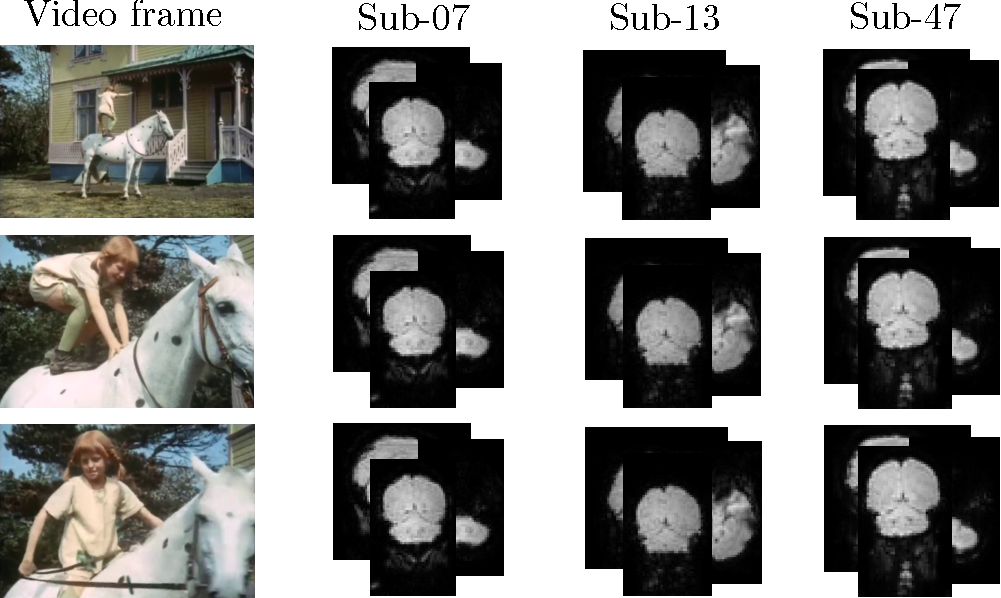
\includegraphics[width=0.8\textwidth]{dataset}
    \caption{The visualization of data from the utilized sample of subjects under examination. Three points in time were selected for example. The video frames are presented in the left-hand section of the figure. The right-hand side of the diagram shows slices of fMRI scans from the relevant time period for three different subjects: 7, 13 and 47. The video frame rate is greater, therefore each fMRI scan is matched with a bunch of video frames.}
    \label{fig:dataset}
\end{figure}

\begin{table}[h!]
\caption{Dataset Description}\label{table:sample}
\begin{tabular}{@{}ccc@{}}
\toprule
Name & Notation & Value \\ 
\midrule
Duration of examination & $t$ & 390 s \\
Video frame rate & $\nu$ & 25 Hz \\
fMRI frame rate & $\mu$ & 1.64 Hz \\
Video dimensions & $W, H, C$ & 640, 480, 3 \\
fMRI dimensions & $X, Y, Z$ & 40, 64, 64 \\
\botrule
\end{tabular}
\end{table}

The sample was divided into training and test samples in the ratio of 70\% and 30\%, respectively.
During the training stage, we obtain an optimal weights matrix $\hat{\mathbf{W}}$, which is then utilized to forecast fMRI images auto-regressively on the test sample.
To measure an image reconstruction quality, we have chosen the MSE, i.e., the sum of squares of deviations between the true and reconstructed images, averaged over all voxels of each image from the test sample.

To reduce the running time of the algorithm, the fMRI image is precompressed
using MaxPool3D layer. Compression ratios of 1, 2, 4 and 8 are considered.
The voxel values are normalized to $[0; 1]$ by the MinMaxScale procedure.
In particular, we calculate the mean and variance on the training sample, and transform the training and test samples using these statistics.

Table~\ref{table:pc} summarizes the specifications of the computer on which the computational experiment was
on which the computational experiment was performed.

\begin{table}[h!]
\caption{PC Specification}\label{table:pc}
\begin{tabular}{@{}cc@{}}
\toprule
Element & Description \\
\midrule
CPU & Intel Core i7-7700 3.6 GHz \\
GPU & NVIDIA GeForce GTX 1060 3 GB \\
RAM & 16 GB 2400 MHz \\
Hard Drive & M.2 SSD \\
OS & Windows 10 \\
\botrule
\end{tabular}
\end{table}

\subsection{Method forecasting example}

Figure~\ref{fig:example} shows slices of the true and reconstructed images from the test sample.
Figure\myfigref{fig:example}{fig:example-c} shows the difference between them.
To demonstrate the performance of the algorithm, the 7th subject was selected, $\Delta t = 5 \text{s}$, compression factor 1, regularization factor
$\alpha = 1000$. The 20th slice along the first coordinate of the 37th image in the sequence was considered.
Since the voxel values are normalized to the segment $[0; 1]$, an error of the order of $10^{-3}$
indicates a fairly accurate prediction.

\begin{figure}[h!]
	\centering
	\subfloat[Test]{\label{fig:example-a}{\includegraphics[width=0.33\textwidth]{sub-07-5-1-1000-37-20-_-_-test.png}}}
	\hfill
	\subfloat[Predicted]{\label{fig:example-b}{\includegraphics[width=0.33\textwidth]{sub-07-5-1-1000-37-20-_-_-predicted.png}}}
	\hfill
	\subfloat[Difference]{\label{fig:example-c}{\includegraphics[width=0.33\textwidth]{sub-07-5-1-1000-37-20-_-_-difference.png}}}
	\caption{\textbf{Slices of fMRI images from the test sample.} The figure presents slices of the true and reconstructed tomographic scan from the test sample and the difference between them. An error on the order of $10^{-3}$ indicates a fairly accurate prediction.}
	\label{fig:example}
\end{figure}

\subsection{Delay time analysis}

In this section, we investigate the dependence of recovery quality on the delay time.
The 47th subject and 4x compression were chosen for the example.
The left graph in Figure~\ref{fig:mse-dt} shows the dependence of the MSE metric
on the delay time $\Delta t$.
The study confirms that the most active part of the brain is the most active part of the brain 
in this examination~--- the occipital lobe.
The other parts contribute noise to the considered dependence.
In the present work, the above-mentioned region is localized, 
as shown in Figure~\ref{fig:local}.
To localize the region, the lower third and the right two thirds of the volumetric
of the tomographic image.

The area highlighted in red is the area that contains the 3\% 
of the most variable voxels in the occipital lobe.
For this purpose, all voxels of the localized area were ordered by 
descending order of the total absolute change in values.
Then 3\% of voxels with the largest changes were selected.
The MSE metric was recalculated exactly on this part of the image.
The corresponding graph is shown on the right side of Figure~\ref{fig:mse-dt}.
There is a more distinct minimum at $\Delta t \approx 5$ seconds. 

This result is highly correlated with the existing medical research~\cite{Bandettini1992}. Specifically, the delay time of 5 seconds is common for the BOLD signal delay in the human brain. Consequently, we set this 5-second value for the hyperparameter $\Delta t$ and keep it constant throughout the forecasting stage of our proposed method.


\begin{figure}[h!]
	\centering
	\subfloat[True]{\label{fig:local-a}{\includegraphics[width=0.33\textwidth]{sub-47-5-1-1000-37-20-_-_-test.png}}}
	\hfill
	\subfloat[Predicted]{\label{fig:local-b}{\includegraphics[width=0.33\textwidth]{sub-47-5-1-1000-37-20-_-_-predicted.png}}}
	\hfill
	\subfloat[Difference]{\label{fig:local-c}{\includegraphics[width=0.33\textwidth]{sub-47-5-1-1000-37-20-_-_-difference.png}}}
	\caption{\textbf{Localization of the most active zone.} The figure indicates that the localized region is the occipital lobe. This area of the brain is responsible for processing visual information, including information during the viewing of a video sequence, which supports the correctness of the localization.}
	\label{fig:local}
\end{figure}

\begin{figure}[h!]
	\centering
	\includegraphics[width=\textwidth]{mse_dt.pdf}
	\caption{\textbf{Dependence of MSE on delay time.} On the left side, the graph does not exhibit any point of minimum. We investigate that calculation on the entire fMRI image is noisy. Therefore, we correct the MSE, localizing the occipital lobe, which leads to the distinctive minimum at 5 seconds (on the right side).}
	\label{fig:mse-dt}
\end{figure}

\subsection{Optimal regularization parameter}

In this section, we investigate the optimal value of the $L_2$ regalurization coefficient in the formula~\eqref{eq8}.
For each compression factor 1, 2, 4, and 8, we calculate the average value of MSE on the test tample.
Averaging over the subjects was performed to construct the graph.
The corresponding plots are shown in the Figure~\ref{fig:mse-alpha}.
The limits of standard deviation are marked.

The graphs show that the optimal value of the coefficient is $\alpha \approx 1000$.
The curve shape is preserved regardless of the compression factor of fMRI images.
Nevertheless, one can see that increasing the compression leads to the MSE increasing.
This is mostly due to the different number of background voxels on the scans.
Specifically, our method has a higher quality on the background, as those values remain constant over time.
In contrast, the use of max pooling for compression results in the higher number of foreground voxels. 

\begin{figure}[h!]
	\centering
	\includegraphics[width=0.65\textwidth]{subs_MSE_alpha.pdf}
	\caption{\textbf{Dependence of MSE metric on regularization parameter $\alpha$ on images from the test sample.} The graphs show that the optimal value of the
coefficient is $\alpha \approx 1000$. Increasing the compression ratio reduces quality due to the lower number of background voxels.}
	\label{fig:mse-alpha}
\end{figure}

\subsection{Effect of image compression ratio on method runtime}

We compare the training time of the model when using different
compression coefficients of fMRI images. Coefficients 1, 2, 4 and 8 are considered.
For each value of the compression ratio, the average value of the model training time for all subjects is calculated.
value of the model training time. The standard deviation is calculated.
The experimental results are summarized in Table~\ref{table:coeffs}.
The running time of the method is significantly reduced when using
pre-compression of fMRI images. 
The experiment with the selection of the optimal regularization coefficient
confirms that the compression of the images does not change the dependences.

\begin{table}[h!]
\caption{Dependence of model training time on compression ratio}\label{table:coeffs}
\begin{tabular}{@{}ccc@{}}
\toprule
Compression coefficient & Mean time, s & Std, s \\
\midrule
1 & 36.3 & 6.1 \\
2 & 6.7 & 0.5 \\
4 & 1.6 & 0.1 \\
8 & 1.4 & 0.3 \\
\botrule
\end{tabular}
\end{table}

\subsection{Analyzing the distribution of model weights}

In order to investigate the explainability of the our proposed model, we plot the model weights distribution.
We average the corresponding weights over all voxels for the 4th subject.
The result is shown in Figure~\ref{fig:w-distr}.
The model weights do not lie in the neighborhood of any particular value, 
that is, their distribution is not degenerate.
This result is quite consistent with reality, because a human being, while viewing
pays attention to certain parts of the frame, such as characters or other details.
other details.

\begin{figure}[h!]
	\centering
	\includegraphics[width=0.65\textwidth]{distribution.pdf}
	\caption{\textbf{Weights vector component distribution.} The model weights are not concentrated around any particular value, indicating a non-degenerate distribution. This suggests that the model is well-trained and captures a diverse range of features.}
	\label{fig:w-distr}
\end{figure}

\subsection{Hypothesis of invariance of model weights with respect to humans}

The hypothesis of invariance of the model weights with respect to the person was tested:
Using one subject's weight matrix to reconstruct another subject's fMRI images.
The MSE metric on the test sample was used.
The results are presented in Table~\ref{table:inv}.
The 4th and 7th subjects were considered. 
The weight matrix of the 4th was used to reconstruct the 7th subject's images.
The MSE values are almost the same.

\begin{table}[h!]
\caption{Testing the hypothesis of invariance of model weights with respect to humans}\label{table:inv}
\begin{tabular}{@{}cccc@{}}
\toprule
Weights matrix & True & Mixed  & Difference \\
\midrule
MSE & $6.3912 \cdot 10^{-5}$ & $6.3911 \cdot 10^{-5}$ & $1.37 \cdot 10^{-9}$ \\
\botrule
\end{tabular}
\end{table}

A similar experiment was conducted for each pair of subjects, with the results presented in Figure~\ref{fig:heatmap}. The heatmap was generated using the following procedure: 
 
For a given subject (represented by a row in the matrix), we first calculated the "true" Mean Squared Error (MSE). Then, we considered another subject (represented by a column in the matrix) and used their weight matrix~\eqref{eq13} to predict the first subject's outcomes. We then calculated the "mixed" MSE and determined the percentage difference between the "true" and "mixed" MSE values. This percentage is what is displayed in the heatmap, essentially representing the Mean Absolute Percentage Error (MAPE) between subjects. 

\begin{figure}[h!]
	\centering
	\includegraphics[width=0.5\textwidth]{heatmap.pdf}
	\caption{\textbf{MAPE of MSE changing when predicting on the mixed weight matrix.} The figure shows the Mean Absolute Percentage Error (MAPE) of predicted MSE between pairs of subjects.
    Each row and column represents a subject.
    "Mixed" MSE uses one subject's weights to predict another's outcomes.
    Positive values indicate "mixed" MSE is greater than the "true" MSE.}
	\label{fig:heatmap}
\end{figure}
 
Positive values in the heatmap indicate that the "mixed" MSE is greater than the "true" MSE, while negative values indicate that the "mixed" MSE is smaller. Ideally, the model should produce only positive deviations. However, Figure~\ref{fig:heatmap} shows some negative values with deviations on the order of 1\%. This can be attributed to the model's simplicity, which affords it high generalization capability. Despite these minor negative deviations, the data do not contradict the hypothesis that the model's weights are invariant with respect to different humans.

\subsection{Correctness of the method using uninformative data}

In this section, we investigate the purpose of using the high-quality image features in the proposed forecasting method. Specifically, we replace the original image features, obtained through the ResNet152 image encoder, with the uninformative ones. This means that we set the matrix $\mathbf{X}$ in the equation~\eqref{eq10}, filling it with values of 1. 

We compare the forecasting results for the original objects-features matrix with the uninformative one. For this purpose, we apply the proposed method auto-regressively to obtain the last fMRI image in the test sequence. To do it, we sum all the predicted differences subsequently to the 1st fMRI image in the test sample, which results in the last image forecasting. The 35th subject was chosen.  

Figure~\ref{fig:recover} shows  slices of the last true and recovered snapshots from the test sample. Figure\myfigref{fig:recover}{fig:recover-c} shows the difference between them. The results on the uninformative ones are demonstrated in Figure~\ref{fig:random}.

The difference between the true and recovered images when working with uninformative data is much higher, which confirms that there is a correlation between the sensor readings and the images from the video sequence. The numerical results are summarized in Table~\ref{table:random}.

\begin{figure}[h!]
	\centering
	\subfloat[True]{\label{fig:recover-a}{\includegraphics[width=0.33\textwidth]{sub-35-5-1-1000--1-20-_-_-recovered-test.png}}}
	\hfill
	\subfloat[Predicted]{\label{fig:recover-b}{\includegraphics[width=0.33\textwidth]{sub-35-5-1-1000--1-20-_-_-recovered-predicted.png}}}
	\hfill
	\subfloat[Difference]{\label{fig:recover-c}{\includegraphics[width=0.33\textwidth]{sub-35-5-1-1000--1-20-_-_-recovered-difference.png}}}
	\caption{\textbf{Slices of fMRI images from the test sample.} Figure shows slices from the ground truth and reconstructed tomographic scan (derived from original video frames using proposed method) along with the differences between them.}
	\label{fig:recover}
\end{figure}

\begin{figure}[h!]
	\centering
	\subfloat[True]{\label{fig:random-a}{\includegraphics[width=0.33\textwidth]{noised_sub-35-5-1-1000--1-20-_-_-recovered-test.png}}}
	\hfill
	\subfloat[Predicted]{\label{fig:random-b}{\includegraphics[width=0.33\textwidth]{noised_sub-35-5-1-1000--1-20-_-_-recovered-predicted.png}}}
	\hfill
	\subfloat[Difference]{\label{fig:random-c}{\includegraphics[width=0.33\textwidth]{noised_sub-35-5-1-1000--1-20-_-_-recovered-difference.png}}}
	\caption{\textbf{Slices of fMRI images from the test sample (uninformative data).} The MSE value for the uninformative sample is larger, which indicates the presence of a correlation between the true data.}
	\label{fig:random}
\end{figure}

\begin{table}[h!]
\caption{Quality of method performance on uninformative data}\label{table:random}
\begin{tabular}{@{}cccc@{}}
\toprule
Data & True & Uninformative & Difference \\
\midrule
MSE     & $3.67 \cdot 10^{-4}$ & $1.39 \cdot 10^{-3}$ & $1.02 \cdot 10^{-3}$ \\
\botrule
\end{tabular}
\end{table}

\section{Discussion}

The results of this study provide valuable insights into the relationship between video sequences and fMRI images, highlighting the potential of linear models in predicting brain activity based on visual stimuli. Our theoretical analysis and empirical findings demonstrate that a linear autoregressive model can effectively capture the correlation between video frames and fMRI images, assuming the Markov property of the fMRI sequence. This approach allows us to predict subsequent fMRI images given the preceding image and the corresponding video frame, thereby reconstructing the entire sequence of magnetic resonance images based on the viewed video.

The findings of our research are closely connected to the broader field of neuroimaging and brain-computer interfaces. While previous studies have often relied on complex transformer models for video prediction tasks, our method offers a simpler yet effective alternative for analyzing the correlation between visual stimuli and brain activity. This simplified approach can be particularly useful in practical applications where detailed analysis is not required.

However, this study has several potential limitations. First, the dataset used in this study, although comprehensive, is relatively small in terms of the number of subjects. Future work should aim to validate the model on larger and more diverse datasets to ensure its generalizability. Second, the linear autoregressive model, while computationally efficient, may not capture the full complexity of the relationship between video stimuli and fMRI images. More sophisticated models, such as deep learning architectures, could potentially improve prediction accuracy but at the cost of increased computational complexity. Third, the spatial and temporal resolution of fMRI is a known limitation, and the model's performance may be affected by the inherent delay in the hemodynamic response. Future work could explore methods to account for this delay more accurately.

Despite these limitations, we believe that our findings contribute to a deeper understanding of the human brain's reaction to external stimuli and provide a basis for future research in this area.

\section{Conclusion}

In this paper, we have presented a comprehensive study of the correlation between video sequences and fMRI images using a linear autoregressive model. Our theoretical analysis and empirical results demonstrate that the proposed model can effectively predict future fMRI images given the preceding image and the corresponding video frame. This approach leverages the Markov property of the fMRI sequence and accounts for the hemodynamic response time, providing valuable insights into the dynamic relationship between visual stimuli and brain activity.

Our findings highlight the potential of linear models in predicting brain activity based on visual stimuli. While the proposed method has limitations, it offers a simplified yet effective approach for analyzing fMRI data in the context of video stimuli. We believe that our results will contribute to the development of more precise studies of the relationship between visual stimuli and brain activity and have implications for the development of practical applications in cognitive neuroscience and brain-computer interfaces. Future work will focus on extending our results to other architectures, improving the model's performance, and validating the method on larger and more diverse datasets.

\section{Declarations}

\subsection*{Acknowledgements}

This research has been financially supported by The Analytical Center for the Government of the Russian Federation (Agreement No. 70-2021-00143 01.11.2021, IGK 000000D730324P540002).

\subsection*{Competing interests}

The authors have no relevant financial or non-financial interests to disclose.

\subsection*{Ethical approval}

The dataset~\cite{Berezutskaya2022} was approved by the Medical Ethical Committee of the University Medical Center Utrecht in accordance with the Declaration of Helsinki (2013).

\bibliography{references}% common bib file
%% if required, the content of .bbl file can be included here once bbl is generated
%%\input sn-article.bbl


\end{document}
